%=======================================================================
%  LeanGrow  --  Conference talk (AI4Math)
%  Beamer presentation to accompany the live Lean code showcases.
%=======================================================================
\documentclass[aspectratio=169]{beamer}

%----------------------------------------------------------------------
%  Theme
%----------------------------------------------------------------------
\usetheme{Madrid}
\usecolortheme{default}
\setbeamertemplate{navigation symbols}{}   % hide navigation clutter
\setbeamertemplate{caption}[numbered]

%----------------------------------------------------------------------
%  Fonts & encoding
%----------------------------------------------------------------------
\usepackage[T1]{fontenc}
\usepackage[utf8]{inputenc}
\usepackage{lmodern}

%----------------------------------------------------------------------
%  Math
%----------------------------------------------------------------------
\usepackage{amsmath}
\usepackage{amssymb}
\usepackage{amsthm}
\usepackage{mathtools}

%----------------------------------------------------------------------
%  Graphics & figures
%----------------------------------------------------------------------
\usepackage{graphicx}
\usepackage{tikz}
\usetikzlibrary{
  arrows.meta,
  positioning,
  calc,
  fit,
  shapes.geometric,
  backgrounds,
  trees,
  graphs,
  decorations.pathreplacing,
  matrix
}
\usepackage{pgfplots}
\pgfplotsset{compat=1.18}

%----------------------------------------------------------------------
%  Code listings (for the Lean showcases)
%  Official Lean setup: listings + lstlean.tex
%  (https://lean-lang.org/documentation/latex-syntax-highlighting/)
%----------------------------------------------------------------------
\usepackage{listings}
\usepackage{xcolor}

\definecolor{keywordcolor}{rgb}{0.7, 0.1, 0.1}   % keywords
\definecolor{tacticcolor}{rgb}{0.0, 0.1, 0.6}    % tactics
\definecolor{commentcolor}{rgb}{0.4, 0.4, 0.4}   % comments
\definecolor{symbolcolor}{rgb}{0.0, 0.1, 0.6}    % symbols
\definecolor{sortcolor}{rgb}{0.1, 0.5, 0.1}      % Sort/Type/Prop
\definecolor{attributecolor}{rgb}{0.7, 0.1, 0.1} % attributes

\def\lstlanguagefiles{lstlean.tex}
\lstset{language=lean}

% Global tweaks on top of lstlean.tex, to suit beamer frames.
\definecolor{leanBg}{RGB}{248,248,248}
\lstset{
  backgroundcolor=\color{leanBg},
  frame=single,
  rulecolor=\color{gray!40},
  showstringspaces=false,
}

%----------------------------------------------------------------------
%  Handy macros
%----------------------------------------------------------------------
\usepackage{booktabs}
\usepackage{hyperref}

\newcommand{\grow}{\texttt{grow}}      % the tactic
\newcommand{\leangrow}{\textsc{LeanGrow}}

%----------------------------------------------------------------------
%  Section divider frames
%  A plain frame showing only the section name, before each section.
%----------------------------------------------------------------------
\AtBeginSection[]{%
  \begin{frame}[plain,noframenumbering]
    \centering
    \vfill
    {\usebeamercolor[fg]{title}\color{keywordcolor}%
      \Huge\bfseries\insertsection\par}
    \vfill
  \end{frame}
}

%======================================================================
%  Title page
%======================================================================
\title[\leangrow]{Aspects of heuristic proof search}


\author[Yves Jäckle]{Yves Jäckle}

\date[AI4Math]{AI4Math Workshop\\Hasso-Plattner-Institute\\ July 2026}

% \titlegraphic{\includegraphics[height=1.5cm]{logo}}  % optional logo

%======================================================================
\begin{document}

%--- Title frame ------------------------------------------------------
\begin{frame}[plain]
  \titlepage
\end{frame}

%--- Outline ----------------------------------------------------------
\begin{frame}{Outline}
  \tableofcontents
\end{frame}

%======================================================================
%  PART I  --  Interactive Theorem Provers and Lean
%======================================================================
\section{Interactive Theorem Provers and Lean}

%--- What is an ITP? --------------------------------------------------
\begin{frame}{Interactive theorem provers}
  An \alert{interactive theorem prover} (ITP, or proof assistant) is
  software for writing machine checkable maths in a nice way.
  \medskip
  \begin{itemize}
    \item The user supplies the definitions, statements \alert{and proofs}
    \item The machine rejects anything that does not \alert{typecheck}
    \item Established systems: \alert{Lean}, Rocq/Coq, Isabelle/HOL, Agda, \dots
  \end{itemize}
  \medskip
  \begin{block}{Lean 4}
    A proof assistant and a full programming language, built on
    \alert{dependent type theory}.
    \begin{itemize}
      \item Lean supports \alert{metaprogramming} : this is how tactics like \grow{} are written
      \item Backed by a large mathematical library, \alert{Mathlib}, and soon \alert{CSlib}
    \end{itemize}
  \end{block}
\end{frame}

%======================================================================
%  PART II  --  A first look at Lean, following 0_Lean.lean
%======================================================================
\section{A first look at Lean}


%--- Nat: types and terms ---------------------------------------------
\begin{frame}[fragile]{The natural numbers}
	
\large{\textbf{Lean by example}}
\\Let's define the natural numbers
	
\begin{lstlisting}
axiom Nat : Type
-- there is a type of objects called *Nat*ural numbers
axiom Nat.zero : Nat
-- zero is a natural number
axiom Nat.succ (n : Nat) : Nat
-- given a natural number, there is a successor for it
\end{lstlisting}
\small{(Normally \texttt{Nat} is an \texttt{inductive} type; here we
	axiomatize the primitives to keep them visible.)}
\\\texttt{axiom} postulates a constant of a given type
\end{frame}

%--- Definitions ------------------------------------------------------
\begin{frame}[fragile]{Definitions name terms}
\begin{lstlisting}
def Nat.one : Nat := Nat.succ Nat.zero   -- defines 1
def Nat.two : Nat := Nat.succ Nat.one    -- defines 2
\end{lstlisting}
  \begin{itemize}
    \item \texttt{def} introduces a new name for a term of a stated type
    \item Lean has nice machinery to translate between litterals and this representation
  \end{itemize}
\end{frame}

%--- Propositions and predicates --------------------------------------
\begin{frame}[fragile]{Propositions as types: the $\leq$ relation}
\begin{lstlisting}
axiom Nat.leq (n m : Nat) : Prop
-- a relation between natural numbers:  n ≤ m

axiom Nat.leq_zero (n : Nat) : Nat.leq Nat.zero n
-- ∀ n, 0 ≤ n

axiom Nat.leq_step (n m : Nat) (h : Nat.leq n m) :
  Nat.leq (Nat.succ n) (Nat.succ m)
-- ∀ n m, n ≤ m → n+1 ≤ m+1
\end{lstlisting}
  \begin{itemize}
    \item \texttt{Prop} is the type of \alert{propositions}
    \item We'll prove all we need from \texttt{leq\_zero} and \texttt{leq\_step}
  \end{itemize}
\end{frame}

%--- myFirstTheorem : staged proof ------------------------------------
\begin{frame}[fragile]{Proofs as terms \hfill (1/3)}
  Goal: construct a term of type $1 \leq 2$.
\begin{lstlisting}
def myFirstTheorem : Nat.leq Nat.one Nat.two := -- 1 ≤ 2
  sorry
\end{lstlisting}
  \begin{itemize}
    \item To \emph{prove} a proposition is to \alert{construct a term} of it as type
    \item The \emph{statement} is the type
    \item The \emph{proof} is the term
    \item \texttt{sorry} stands in for the missing term we'll fill out
  \end{itemize}
\end{frame}

\begin{frame}[fragile]{Proofs as terms \hfill (2/3)}
  $1 \leq 2$ should follow from $0 \leq 1$ via \texttt{leq\_step}.
\begin{lstlisting}
def myFirstTheorem : Nat.leq Nat.one Nat.two :=
  Nat.leq_step   -- 1 ≤ 2 will follow from 0 ≤ 1
    Nat.zero     -- since 1 is 0+1
    Nat.one      -- and 2 is 1+1
    sorry        -- remaining argument = remaining goal:  0 ≤ 1
\end{lstlisting}
  \begin{itemize}
    \item Applying \texttt{leq\_step} reduces the goal:
          it now suffices to prove subgoal $0 \leq 1$
          \\This is a \alert{backward step}
    \item The two arguments  $n := 0$, $m := 1$ determine the next goal
    	  \\The third arguments type \textit{depends} on the previous arguments
  \end{itemize}
\end{frame}

\begin{frame}[fragile]{Proofs as terms \hfill (3/3)}
  The last goal $0 \leq 1$ is exactly \texttt{leq\_zero}.
\begin{lstlisting}
def myFirstTheorem : Nat.leq Nat.one Nat.two :=
  Nat.leq_step Nat.zero Nat.one
    (Nat.leq_zero Nat.one)   -- proves 0 ≤ 1
\end{lstlisting}
  \begin{itemize}
    \item No \texttt{sorry} left: the term is complete and typechecks.
    \item Had we written \texttt{Nat.leq\_zero Nat.two} instead, 
       \\Lean would have thrown an error
  \end{itemize}
\end{frame}


%--- Recursion / induction --------------------------------------------
\begin{frame}[fragile]{Recursion}
\begin{lstlisting}
axiom Nat.recursion (n : Nat) (expr : Nat -> Sort u)
	(base : expr Nat.zero)
	(step : ∀ m, expr m -> expr (Nat.succ m)) : expr n
\end{lstlisting}
One principle, two readings:
\begin{itemize}
	\item \texttt{expr : Nat $\to$ \alert{Prop}} $\Rightarrow$
	\alert{induction} (prove a statement for all $n$).
	\item \texttt{expr : Nat $\to$ \alert{Type}} $\Rightarrow$
	\alert{recursion} (define a function on $n$).
\end{itemize}
\end{frame}

%--- Second theorem --------------------------------------------
\begin{frame}[fragile]{Recursion}
	\begin{lstlisting}
def mySecondTheorem (n : Nat) : Nat.leq n (Nat.succ n) := -- n ≤ n+1
  Nat.recursion -- induction
    n (fun x => Nat.leq x (Nat.succ x))
	(base := Nat.leq_zero (Nat.succ Nat.zero)) -- 0 ≤ 1
	(step := -- ∀ n, n ≤ n+1 → n+1 ≤ (n+1)+1
	  fun n ih => -- ∀ n : ℕ, ih : n ≤ n+1
		Nat.leq_step n (Nat.succ n) ih
	)
	\end{lstlisting}
\begin{itemize}
	\item Named arguments (ex: \texttt{(base := \ldots)}) for clarity
	\item Anonymous functions \texttt{fun}
	\item To prove $\forall$ display function that maps objects/hypotheses to a proof
\end{itemize}
\end{frame}

%--- Second theorem with forward step--------------------------------------------
\begin{frame}[fragile]{Recursion}
\begin{lstlisting}
def mySecondTheorem (n : Nat) : Nat.leq n (Nat.succ n) := -- n ≤ n+1
  have fwd : Nat.leq Nat.zero (Nat.succ Nat.zero) := -- 0 ≤ 1
    Nat.leq_zero (Nat.succ Nat.zero)
  -- We now have 0 ≤ 1 in context
  Nat.recursion -- induction
	n (fun x => Nat.leq x (Nat.succ x))
	(base := fwd) -- matches subgoal
	(step := -- ∀ n, n ≤ n+1 → n+1 ≤ (n+1)+1
	  fun n ih => -- ∀ n : ℕ, ih : n ≤ n+1
		Nat.leq_step n (Nat.succ n) ih
	)
\end{lstlisting}
\begin{itemize}
	\item \texttt{have} adds fact proven from current hypotheses and facts
	\item This is a \alert{forward step}
\end{itemize}
\end{frame}

%--- Equality ---------------------------------------------------------
\begin{frame}[fragile]{Equality and rewriting}
Defining equality:
\begin{lstlisting}
axiom Eq {T : Sort u} (a b : T) : Prop
-- the proposition  a = b

axiom Eq.refl {T : Sort u} (a : T) : Eq a a
-- reflexivity:  a = a

axiom Eq.rewrite {T : Sort u} (a b : T) (eq : Eq a b)
  (expr : T -> Sort v) (h : expr a) : expr b
-- from a = b and a expression containing a, get the same with b
\end{lstlisting}
  \begin{itemize}
    \item \texttt{\{T : Sort u\}} is an \alert{implicit} argument (in braces):
          Lean infers it.
    \item \texttt{Eq.rewrite} is the \alert{substitution principle}
  \end{itemize}
\end{frame}

%--- Eq.symm : staged proof -------------------------------------------
\begin{frame}[fragile]{Symmetry of equality \hfill (1/2)}
  Goal: from \texttt{eq : a = b}, produce a proof of $b = a$.
\begin{lstlisting}
def Eq.symm {T : Sort u} (a b : T) (eq : Eq a b) : Eq b a :=
  sorry
\end{lstlisting}
Challenge: solve this faster then we move to the next slide

\end{frame}

\begin{frame}[fragile]{Symmetry of equality \hfill (2/2)}
\begin{lstlisting}
def Eq.symm {T : Sort u} (a b : T) (eq : Eq a b) : Eq b a :=
  -- b = a will follow from a = a after rewriting b into a
  Eq.rewrite a b eq            
    (expr := fun x => Eq x a)  -- the expression 
    (h := Eq.refl a)           -- supply expr a, i.e. a = a, via reflexivity
\end{lstlisting}

\end{frame}



%%--- Nat.add ----------------------------------------------------------
%\begin{frame}[fragile]{Defining addition by recursion}
%\begin{lstlisting}
%def Nat.add (n m : Nat) : Nat :=
%  Nat.recursion n (fun _ => Nat)   -- recurse on n
%    (base := m)                    -- 0 + m = m
%    (step := fun k res_k => Nat.succ res_k)
%                                   -- (k+1) + m = (k + m) + 1
%\end{lstlisting}
%  \begin{itemize}
%    \item Here \texttt{expr} is the constant \texttt{Nat}, so this is genuine
%          \alert{recursion}: we are defining a function.
%    \item \texttt{res\_k} is the result already computed for \texttt{k}.
%  \end{itemize}
%\end{frame}
%
%%--- Computation rules ------------------------------------------------
%\begin{frame}[fragile]{The computation rules}
%\begin{lstlisting}
%axiom Nat.recursion_base ... :
%  Eq (Nat.recursion Nat.zero expr base step) base
%axiom Nat.recursion_step ... :
%  Eq (Nat.recursion (Nat.succ n) expr base step) (step n recu)
%
%def Nat.add_zero (n : Nat) : Eq (Nat.add Nat.zero n) n :=
%  Nat.recursion_base
%def Nat.add_succ (n m : Nat) : 
%  Eq (Nat.add (Nat.succ n) m) (Nat.succ (Nat.add n m)) :=
%    Nat.recursion_step
%\end{lstlisting}
%  \begin{itemize}
%    \item The recursor's \alert{defining equations}, packaged as equalities.
%    \item Lean has them built-in as $\iota$ (iota) \alert{reduction}
%  \end{itemize}
%\end{frame}
%
%%--- mySecondTheorem : the payoff, staged -----------------------------
%\begin{frame}[fragile]{Putting it together: $n \leq n + m$ \hfill (1/4)}
%
%\large{\textbf{Grand finale of the introduction}}
%
%\begin{lstlisting}
%def mySecondTheorem (n m : Nat) : Nat.leq n (Nat.add n m) :=
%  sorry   -- n ≤ n + m
%\end{lstlisting}
%  \begin{itemize}
%    \item We prove it by \alert{induction on $n$} --- i.e.\ \texttt{Nat.recursion}
%          with \\\texttt{expr := fun n => n $\leq$ n + m}.
%    \item This leaves two goals: a \alert{base} case and a \alert{step}.
%  \end{itemize}
%\end{frame}
%
%\begin{frame}[fragile]{Putting it together: $n \leq n + m$ \hfill (2/4)}
%
%
%\begin{lstlisting}
%def mySecondTheorem (n m : Nat) : Nat.leq n (Nat.add n m) :=
%  Nat.recursion n (fun n => Nat.leq n (Nat.add n m))
%    (base := sorry)   -- 0 ≤ 0 + m
%    (step := sorry)   -- ∀ k, k ≤ k+m → k+1 ≤ (k+1)+m
%\end{lstlisting}
%  \begin{itemize}
%    \item The base case is immediate from \texttt{leq\_zero}.
%    \item The step is where the real work --- and a rewrite --- happens.
%  \end{itemize}
%\end{frame}
%
%\begin{frame}[fragile]{Putting it together: $n \leq n + m$ \hfill (3/4)}
%\begin{lstlisting}
%    (base := Nat.leq_zero (Nat.add Nat.zero m))   -- 0 ≤ 0+m
%    (step := fun k step =>
%      -- hypothesis  step : k ≤ k+m
%      have tmp : Nat.leq (Nat.succ k) (Nat.succ (Nat.add k m)) :=
%        Nat.leq_step k (Nat.add k m) step   
%      -- We've just shown k+1 ≤ (k+m)+1
%      sorry)   -- goal:  k+1 ≤ (k+1)+m
%\end{lstlisting}
%  \begin{itemize}
%    \item \texttt{leq\_step} on the hypothesis gives $k{+}1 \leq (k{+}m){+}1$
%          \\In proof search, this is a \alert{forward step}
%    \item But the goal wants $(k{+}1){+}m$ on the right
%  \end{itemize}
%\end{frame}
%
%\begin{frame}[fragile]{Putting it together: $n \leq n + m$ \hfill (4/4)}
%  Rewrite $(k{+}m){+}1 = (k{+}1){+}m$ using \texttt{add\_succ} (in reverse order).
%\begin{lstlisting}
%      -- show  k+1 ≤ (k+1)+m from k+1 ≤ (k+m)+1
%      Eq.rewrite (Nat.succ (Nat.add k m)) (Nat.add (Nat.succ k) m)
%        (eq := Eq.symm _ _ (Nat.add_succ k m)) -- show (k+m)+1 = (k+1)+m
%        (h := tmp)   -- we already have this as a forward step
%\end{lstlisting}
%  \begin{itemize}
%    \item \texttt{add\_succ} gives $(k{+}1){+}m = (k{+}m){+}1$; \texttt{Eq.symm}
%          flips it to the direction we need.
%    \item \texttt{Eq.rewrite} transports \texttt{tmp} to the goal --- proof
%          complete, no \texttt{sorry} remaining. \qedhere
%  \end{itemize}
%\end{frame}

%======================================================================
%  PART III  --  Proof search, the big picture
%======================================================================
\section{Proof search: the big picture}

%--- Backward search, conceptually ------------------------------------
\begin{frame}{Backward search: many roads out of a goal}
  Recall a \alert{backward step} turns a goal into (zero or more) subgoals.
  \\[.4em]
  Take the goal $n \leq n+m$. Several backward steps apply:
  \medskip
  \begin{itemize}
    \item[\textcolor{sortcolor}{$\blacktriangleright$}]
      \texttt{Nat.recursion} (induction on $n$): splits into a
      \alert{base} $0 \leq 0+m$ \emph{and} a \alert{step}
      $k \leq k{+}m \,\vdash\, k{+}1 \leq (k{+}1){+}m$.
      \\{\footnotesize This is a useful step.}
    \item[\textcolor{black!45}{$\blacktriangleright$}]
      rewrite with \texttt{Nat.add\_comm} $(a+b = b+a)$: new goal
      $n \leq m+n$.
      \\{\footnotesize Perfectly legal --- but gets us nowhere (here).}
    \item[\textcolor{keywordcolor}{$\blacktriangleright$}]
      \texttt{le\_of\_lt} $(a < b \to a \leq b)$: new goal $n < n+m$.
      \\{\footnotesize A dead end --- it is \alert{false} when $m = 0$.}
  \end{itemize}
  \medskip
  At every goal there are \alert{many choices}, and some lead nowhere.
\end{frame}

%--- AND-OR tree ------------------------------------------------------
\begin{frame}{The search space is an AND--OR tree}
  \begin{center}
  \resizebox{\linewidth}{!}{%
  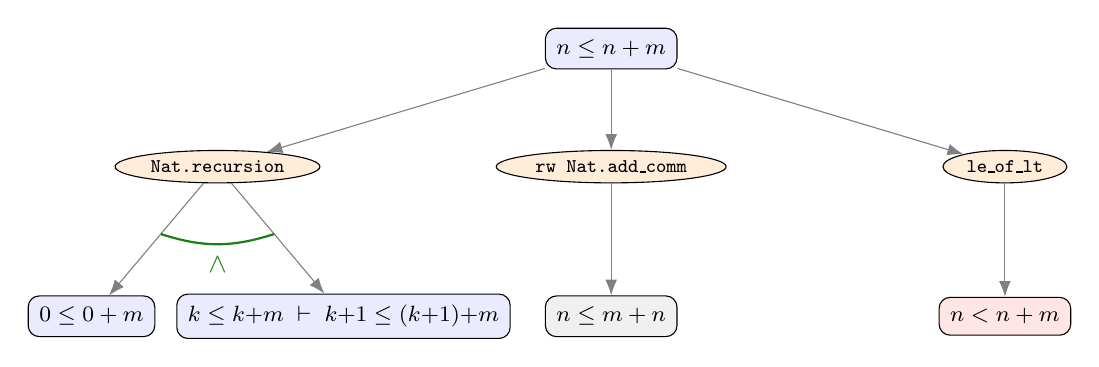
\begin{tikzpicture}[
    every node/.style={font=\footnotesize},
    goal/.style={draw, rounded corners, fill=blue!8, align=center, inner sep=4pt},
    dead/.style={draw, rounded corners, fill=red!10, align=center, inner sep=4pt},
    useless/.style={draw, rounded corners, fill=black!6, align=center, inner sep=4pt},
    bwstep/.style={draw, ellipse, fill=orange!15, inner sep=2pt, font=\ttfamily\scriptsize},
    ed/.style={-{Latex[length=2mm]}, gray}
  ]
    % root goal (OR node)
    \node[goal] (G) {$n \leq n+m$};
    % backward steps (the OR alternatives)
    \node[bwstep] (s1) at (-5.0,-1.5) {Nat.recursion};
    \node[bwstep] (s2) at ( 0.0,-1.5) {rw Nat.add\_comm};
    \node[bwstep] (s3) at ( 5.0,-1.5) {le\_of\_lt};
    \draw[ed] (G) -- (s1);
    \draw[ed] (G) -- (s2);
    \draw[ed] (G) -- (s3);
    % subgoals
    \node[goal]    (b) at (-6.6,-3.4) {$0 \leq 0+m$};
    \node[goal]    (k) at (-3.4,-3.4) {$k \leq k{+}m \;\vdash\; k{+}1 \leq (k{+}1){+}m$};
    \node[useless] (c) at ( 0.0,-3.4) {$n \leq m+n$};
    \node[dead]    (l) at ( 5.0,-3.4) {$n < n+m$};
    \draw[ed] (s1) -- (b);
    \draw[ed] (s1) -- (k);
    \draw[ed] (s2) -- (c);
    \draw[ed] (s3) -- (l);
    % AND arc under Nat.recursion
    \draw[thick, sortcolor]
      ($(s1)!0.45!(b)$) to[bend right=18]
      node[below=1pt]{\normalsize$\wedge$} ($(s1)!0.45!(k)$);
  \end{tikzpicture}}
  \end{center}
  \begin{itemize}
    \item \alert{OR node} (a \emph{goal}): proven if \emph{some} applicable step
          is proven
    \item \alert{AND node} (a \emph{step}): proven only if \emph{all} the
          subgoals it produces are proven
  \end{itemize}
\end{frame}

%--- grow / Aesop / sandbox -------------------------------------------
\begin{frame}[fragile]{Search tactics}
\grow{} explores this AND--OR tree, in the spirit of \alert{Aesop}
\begin{lstlisting}
theorem test (l L : List Nat) (h : (l ++ L).length = 42) :
  (l.length + L.length) = 42 := by
	grows
\end{lstlisting}
Our running examples live in the world of \alert{linked lists}: 
\begin{itemize}
	\item \texttt{length} (number of entries)
	\item \texttt{dedup} (removing duplicates)
	\item sublists (\texttt{<+}) (same order, same multiplicity)
\end{itemize}




  
\end{frame}

%--- Example: test ----------------------------------------------------
\begin{frame}[fragile]{Example 1: close to the human proof}
In our examples we restrict search to a small set of lemmas
\begin{lstlisting}
def stdSanbox := #[`List.dedup_cons_of_mem', `List.length_append,
	`List.mem_dedup, `List.dedup_sublist, `List.dedup_subset,
	`List.dedup_idem, `List.length_erase_le, `List.Perm.dedup, ...]
grow_load_sandbox stdSanbox ; elimSandbox ; funIndSandbox
\end{lstlisting}
\grow{} finds a term close to what a user would write:
\begin{lstlisting}
theorem test : ∀ (l L : List ℕ),
    (l ++ L).length = 42 → l.length + L.length = 42 :=
fun l L h => (fun t => Eq.symm (Eq.symm length_append) ▸ t) h
\end{lstlisting}
Close to output of source language: \texttt{rw [$\leftarrow$ length\_append]; exact h}
\end{frame}

%--- Example: test' ---------------------------------------------------
\begin{frame}[fragile]{Example 2: a proof with a messy term}
\begin{lstlisting}
theorem test' (l : List Nat) : l.dedup <+ l := by
  grows        -- apply dedup_sublist
\end{lstlisting}
  \grow{} succeeds, but the term it finds is \alert{needlessly complicated}:
\begin{lstlisting}
theorem test' : ∀ (l : List ℕ), l.dedup <+ l :=
fun l =>
  let g.1 := dedup_sublist l;   -- the useful forward step
  let g.2 := dedup_subset l;    -- a useless forward step
  (fun t.0 t.1 => rec (motive := fun x =>
      x.dedup <+ x → x.dedup.Subset x → x.dedup <+ x)
    t.0 t.1 l g.1 g.2)
    (fun g.3 g.4 => g.3) (fun g.5 g.6 g.7 g.8 g.9 => g.8)
\end{lstlisting}
\end{frame}

%--- Example: test' ---------------------------------------------------
\begin{frame}[fragile]{Example 2: a proof with a messy term}
\begin{lstlisting}
theorem test' : ∀ (l : List ℕ), l.dedup <+ l :=
fun l =>
  let g.1 := dedup_sublist l;   -- the useful forward step
  let g.2 := dedup_subset l;    -- a useless forward step
  (fun t.0 t.1 => rec (motive := fun x =>
       x.dedup <+ x → x.dedup.Subset x → x.dedup <+ x)
     t.0 t.1 l g.1 g.2)
     (fun g.3 g.4 => g.3) (fun g.5 g.6 g.7 g.8 g.9 => g.8)
\end{lstlisting}
\begin{itemize}
\item show result as forward step
\item make useless forward step
\item show \texttt{x.dedup <+ x → x.dedup.Subset x → x.dedup <+ x} by induction
\item base and step are the hypothesis
\item apply this to our forward steps to get result
\end{itemize}
\end{frame}


%--- Challenges ---------------------------------------------------
\begin{frame}[fragile]{Aspects of proof search}
What are the aspects of proof search ?
\begin{itemize}
	\item Target lean source or \texttt{Lean.Expr}
	\item Allowed steps and tools: forward steps, induction, rewriting, tactics
	\item Find relevant lemmata and relevant steps
	\item Beyond our scope: find relevant definitions and statements to study
	\item Make it bug free and make it scale
\end{itemize}
\end{frame}

%======================================================================
%  PART IV  --  Rewriting
%======================================================================
\section{Rewriting}

%--- Motivation: correct terms ----------------------------------------
\begin{frame}[fragile]{First aspect: the search must build \emph{correct terms}}
``Make it bug free''
\begin{itemize}
\item The whole point of Lean is that a proof is a \alert{term the kernel
      checks}
\item Search steps must assemble into a type-correct term
\end{itemize}

Goal: rewrite $y + x$ into $x + y$ underneath two binders

\begin{lstlisting}
example : (fun x y : Nat => y + x) = Nat.add := by
	rw [Nat.add_comm]        -- FAILS: rw won't rewrite under fun
	
example : (fun x y : Nat => y + x) = Nat.add := by
	simp_rw [Nat.add_comm]   -- succeeds
	-- (fun x y : Nat => x + y) = Nat.add
	rfl
\end{lstlisting}

\begin{itemize}
	\item \texttt{rw} refuses to apply under a binder.
	\item \texttt{simp\_rw} allows it as part of the simplification
\end{itemize}

\end{frame}

%--- Conditional rewriting: both fail ---------------------------------
\begin{frame}[fragile]{Pitfall: rewriting with a side condition}
\begin{lstlisting}[basicstyle=\ttfamily\scriptsize]
#check Nat.add_div_left
-- Nat.add_div_left (a : ℕ) {b : ℕ} (H : 0 < b) : (b + a) / b = a / b + 1

example (a : Nat) :
    (fun (b : Nat) (h : 1 < b+1) => (b + a) / b) = (fun _ _ => 42) := by
  rw [Nat.add_div_left]        -- FAILS

example (a : Nat) :
    (fun (b : Nat) (h : 1 < b+1) => (b + a) / b) = (fun _ _ => 42) := by
  simp_rw [Nat.add_div_left]   -- FAILS, even though it is @[simp]
\end{lstlisting}
  \begin{itemize}
    \item The lemma carries a \alert{side condition} $0 < b$
    \item \grow{} implements a solution to allow this rewrite
  \end{itemize}
\end{frame}

%--- Conditional rewriting: by hand -----------------------------------
\begin{frame}[fragile]{Doing it by hand: thread the side condition}
The big idea:
\begin{lstlisting}[basicstyle=\ttfamily\scriptsize]
example (a : Nat) :
    (fun (b : Nat) (h : 1 < b+1) => (b + a) / b) = (fun _ _ => 42) :=
  have inside (b : Nat) (h : 1 < b+1) (ng : 1 < b+1 → 0 < b) :
    (b + a) / b = a / b + 1 :=
      Nat.add_div_left a (ng h)
  have first_binder (b : Nat) (ng : 1 < b+1 → 0 < b) :
    (fun (h : 1 < b+1) => (b + a) / b) = (fun _ => a / b + 1) :=
      funext (fun h => inside b h ng)
  have second_binder (ng : ∀ b, 1 < b+1 → 0 < b) :
    (fun b (h : 1 < b+1) => (b + a) / b) = (fun b _ => a / b + 1) :=
      funext (fun b => first_binder b (ng b))
  by
  refine @Eq.ndrec _ _ (fun p => p = (fun (b : Nat) (h : 1 < b+1) => 42))
    ?newgoal_main _ (second_binder ?newgoal_cond).symm
  · dsimp
    sorry -- ⊢ (fun b x => a / b + 1) = fun b h => 42
  · sorry -- ⊢ ∀ (b : ℕ), 1 < b + 1 → 0 < b
\end{lstlisting}

\end{frame}

%--- Dependencies: both fail ------------------------------------------
\begin{frame}[fragile]{Pitfall: rewriting inside a dependent type}
Next issue:
\begin{lstlisting}[basicstyle=\ttfamily\scriptsize]
def Fin.isNonZero (n : Nat) (x : Fin (n+1)) := x ≠ 0

example (n m : Nat) (x : Fin (n+m + 1)) :
    x.isNonZero (n+m) → ∃ y : Fin (m+n + 1), y.isNonZero (m+n) := by
  rw [Nat.add_comm]        -- FAILS

example (n m : Nat) (x : Fin (n+m + 1)) :
    x.isNonZero (n+m) → ∃ y : Fin (m+n + 1), y.isNonZero (m+n) := by
  simp_rw [Nat.add_comm]   -- FAILS
\end{lstlisting}
  \begin{itemize}
    \item Pattern \texttt{n+m} appears inside the \alert{dependent type}
          \texttt{Fin (n+m+1)} -- the type of \texttt{x}.
    \item Usual rewrite-term is \alert{not type correct} : $x$'s type is not rewritten
  \end{itemize}
\end{frame}

%--- Dependencies: by hand --------------------------------------------
\begin{frame}[fragile]{Doing it by hand: revert, rewrite, reintroduce}
A solution is to \alert{revert}:
\begin{lstlisting}[basicstyle=\ttfamily\scriptsize]
example (n m : Nat) (x : Fin (n+m + 1)) :
    x.isNonZero (n+m) → ∃ y : Fin (m+n + 1), y.isNonZero (m+n) :=
  have reverted : ∀ (x : Fin (n+m + 1)),
      x.isNonZero (n+m) → ∃ y : Fin (m+n + 1), y.isNonZero (m+n) := by
    refine @Eq.ndrec _ _
      (fun p => ∀ (x : Fin (p + 1)),
        x.isNonZero p → ∃ y : Fin (m+n + 1), y.isNonZero (m+n))
      ?newgoal
      _ (Nat.add_comm m n)
    dsimp
    intro x
    -- ⊢ Fin.isNonZero (m + n) x → ∃ y, Fin.isNonZero (m + n) y
    intro H
    use x
  reverted x
\end{lstlisting}
Much more term building fun to be had!

\end{frame}

%======================================================================
%  PART V  --  Set-tries
%======================================================================
\section{Set-tries}

%--- Motivation -------------------------------------------------------
\begin{frame}{Set-tries: taking forward steps efficiently}
  \begin{itemize}
    \item A \alert{forward step} applies a theorem whose hypotheses are all
          present in our local context.
    \item So we constantly ask: given the facts we currently have, \alert{which
          theorems have all of their hypotheses available?}
  \end{itemize}
  \medskip
  \begin{block}{Abstractly}
    Give:
    \begin{itemize}
    	\item family of \alert{target sets} (each theorem's hypotheses)
    	\item a \alert{query set} (our current facts)
    \end{itemize}
    report every target set that is $\subseteq$ the query set.
  \end{block}
  \medskip
  A \alert{set-trie} is a data-structure to do this efficiently.
\end{frame}

%--- Set-trie example (MaRDI slide, with the ∈ -> ∉ fix) --------------
\begin{frame}{Sharing common hypotheses}
  \begin{center}
  \resizebox{\linewidth}{!}{%
  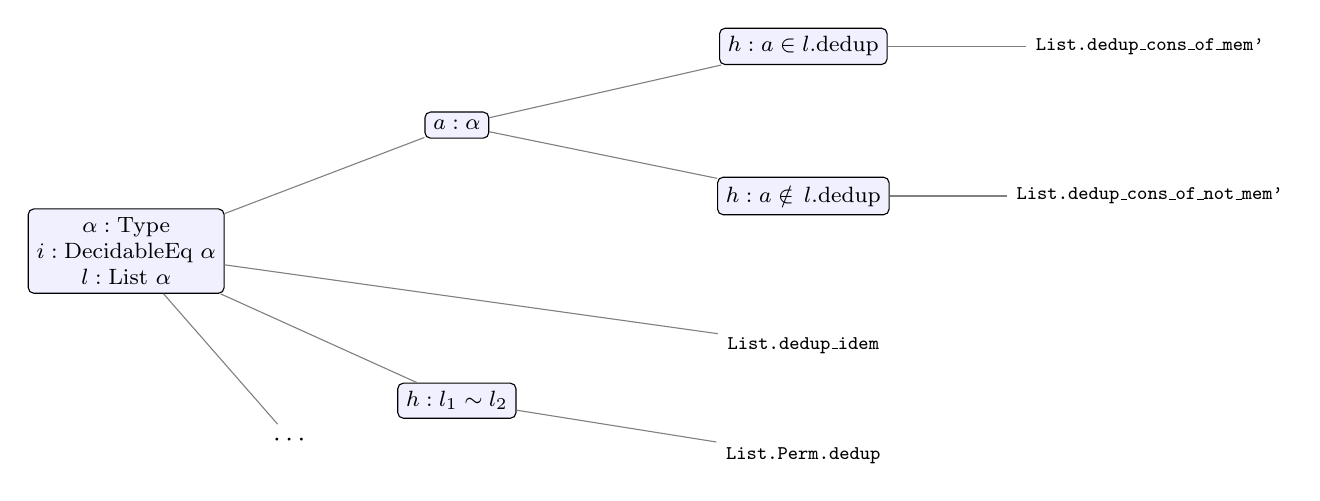
\begin{tikzpicture}[
    bx/.style={draw, rounded corners=2pt, fill=blue!6, align=center,
               inner sep=3pt, font=\footnotesize},
    lf/.style={font=\ttfamily\scriptsize},
    ed/.style={-, gray}
  ]
    \node[bx] (root) at (0,0)
      {$\alpha : \mathrm{Type}$\\ $i : \mathrm{DecidableEq}\ \alpha$\\
       $l : \mathrm{List}\ \alpha$};
    \node[bx] (a)    at (4.2, 1.6) {$a : \alpha$};
    \node[bx] (perm) at (4.2,-1.9) {$h : l_1 \sim l_2$};
    \node[bx] (mem)  at (8.6, 2.6) {$h : a \in l.\mathrm{dedup}$};
    \node[bx] (nmem) at (8.6, 0.7) {$h : a \notin\, l.\mathrm{dedup}$};
    \node[lf] (memL)  at (13.0, 2.6) {List.dedup\_cons\_of\_mem'};
    \node[lf] (nmemL) at (13.0, 0.7) {List.dedup\_cons\_of\_not\_mem'};
    \node[lf] (idem)  at (8.6,-1.2) {List.dedup\_idem};
    \node[lf] (pdd)   at (8.6,-2.6) {List.Perm.dedup};
    \node (dots) at (2.1,-2.4) {$\cdots$};
    \draw[ed] (root)--(a); \draw[ed] (root)--(perm); \draw[ed] (root)--(dots);
    \draw[ed] (a)--(mem); \draw[ed] (a)--(nmem);
    \draw[ed] (mem)--(memL); \draw[ed] (nmem)--(nmemL);
    \draw[ed] (root)--(idem); \draw[ed] (perm)--(pdd);
  \end{tikzpicture}}
  \end{center}
  A root-to-leaf path lists the hypotheses a theorem needs.
\end{frame}

%--- Set-trie example (MaRDI slide, with the ∈ -> ∉ fix) --------------
\begin{frame}{Sharing common hypotheses}
\begin{center}
	\resizebox{0.7\linewidth}{!}{%
		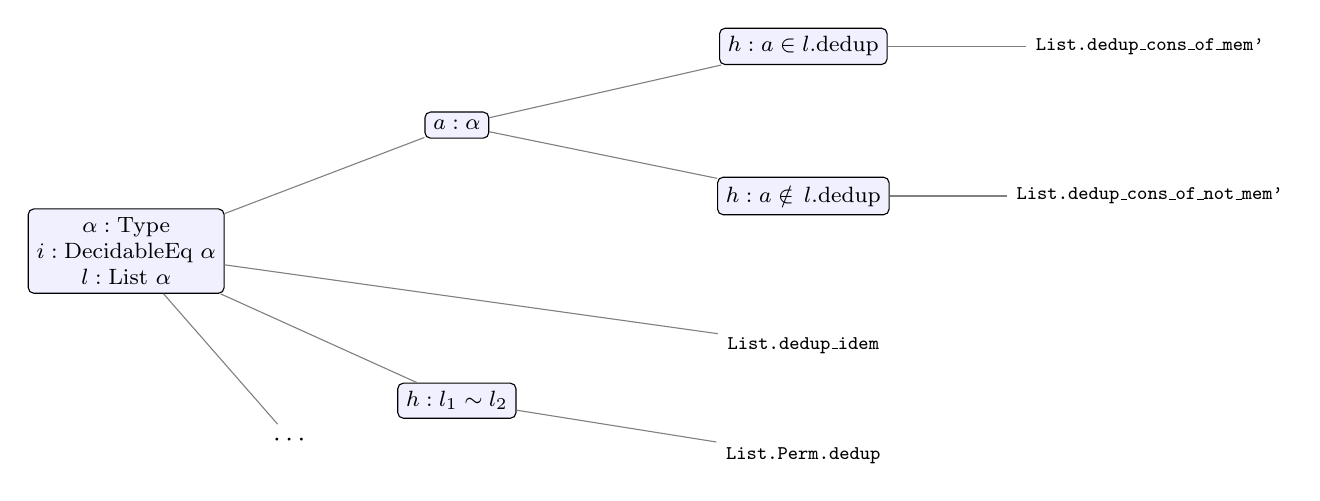
\begin{tikzpicture}[
			bx/.style={draw, rounded corners=2pt, fill=blue!6, align=center,
				inner sep=3pt, font=\footnotesize},
			lf/.style={font=\ttfamily\scriptsize},
			ed/.style={-, gray}
			]
			\node[bx] (root) at (0,0)
			{$\alpha : \mathrm{Type}$\\ $i : \mathrm{DecidableEq}\ \alpha$\\
				$l : \mathrm{List}\ \alpha$};
			\node[bx] (a)    at (4.2, 1.6) {$a : \alpha$};
			\node[lf] (idem)  at (8.6,-1.2) {List.dedup\_idem};
			\node[bx] (perm) at (4.2,-1.9) {$h : l_1 \sim l_2$};
			\node[bx] (mem)  at (8.6, 2.6) {$h : a \in l.\mathrm{dedup}$};
			\node[bx] (nmem) at (8.6, 0.7) {$h : a \notin\, l.\mathrm{dedup}$};
			\node[lf] (memL)  at (13.0, 2.6) {List.dedup\_cons\_of\_mem'};
			\node[lf] (nmemL) at (13.0, 0.7) {List.dedup\_cons\_of\_not\_mem'};
			\node[lf] (pdd)   at (8.6,-2.6) {List.Perm.dedup};
			\node (dots) at (2.1,-2.4) {$\cdots$};
			\draw[ed] (root)--(a); \draw[ed] (root)--(perm); \draw[ed] (root)--(dots);
			\draw[ed] (a)--(mem); \draw[ed] (a)--(nmem);
			\draw[ed] (mem)--(memL); \draw[ed] (nmem)--(nmemL);
			\draw[ed] (root)--(idem); \draw[ed] (perm)--(pdd);
	\end{tikzpicture}}
\end{center}
\begin{itemize}
\item In \grow{} we consider non-inferable hypotheses only (sinks)
\item Note the term dependence, even among sinks
\item Subsets of hypotheses (at set-trie nodes) can be queried efficiently via a \alert{path index}
\item Larger example in code
\end{itemize} 
\end{frame}

%--- Greedy building --------------------------------------------------
\begin{frame}{Building a set-trie: a greedy heuristic}
  Goal: a trie whose total key size (summed over nodes) is small.
  \\Family $\{\{a,b,x\},\{a,c,x\},\{c,d\},\{c,e,y\},\{e,f,y\}\}$. 
  \begin{center}
  \resizebox{0.98\linewidth}{!}{%
  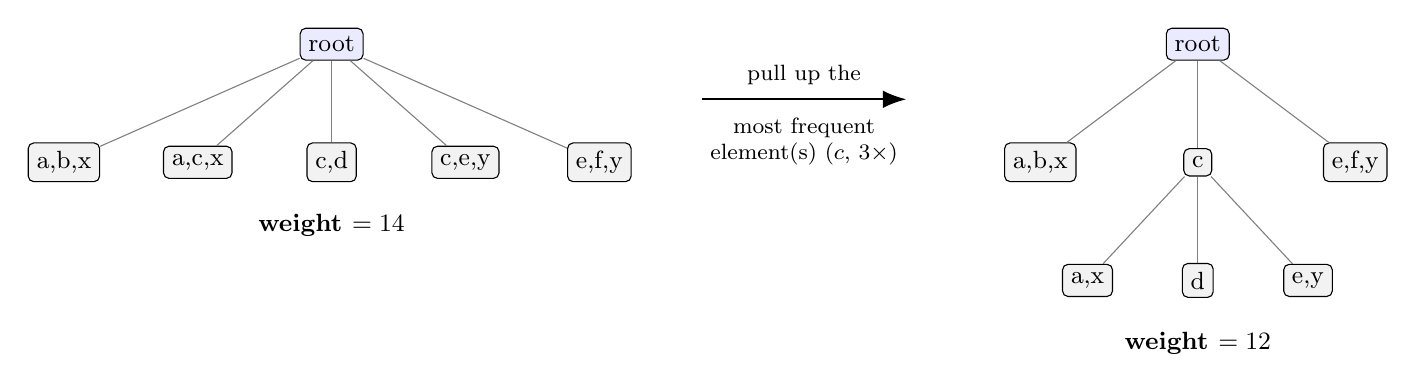
\begin{tikzpicture}[
    nd/.style={draw, rounded corners=2pt, fill=black!5, inner sep=3pt, font=\small},
    rt/.style={draw, rounded corners=2pt, fill=blue!8, inner sep=3pt, font=\small},
    ed/.style={-, gray}
  ]
    % ---- flat trie, weight 14 ----
    \node[rt] (r) at (0,0) {root};
    \node[nd] (n1) at (-3.4,-1.5) {a,b,x};
    \node[nd] (n2) at (-1.7,-1.5) {a,c,x};
    \node[nd] (n3) at ( 0.0,-1.5) {c,d};
    \node[nd] (n4) at ( 1.7,-1.5) {c,e,y};
    \node[nd] (n5) at ( 3.4,-1.5) {e,f,y};
    \foreach \n in {n1,n2,n3,n4,n5} \draw[ed] (r)--(\n);
    \node[font=\small\bfseries] at (0,-2.3) {weight $= 14$};
    % ---- arrow ----
    \node[font=\footnotesize, align=center] at (6.0,-0.9)
      {pull up the\\\\most frequent\\element(s) ($c$, $3\times$)};
    \draw[-{Latex[length=3mm]}, thick] (4.7,-0.7) -- (7.3,-0.7);
    % ---- greedy trie, weight 12 ----
    \node[rt] (R) at (11.0,0) {root};
    \node[nd] (m1) at ( 9.0,-1.5) {a,b,x};
    \node[nd] (mc) at (11.0,-1.5) {c};
    \node[nd] (m5) at (13.0,-1.5) {e,f,y};
    \draw[ed] (R)--(m1); \draw[ed] (R)--(mc); \draw[ed] (R)--(m5);
    \node[nd] (c1) at ( 9.6,-3.0) {a,x};
    \node[nd] (c2) at (11.0,-3.0) {d};
    \node[nd] (c3) at (12.4,-3.0) {e,y};
    \draw[ed] (mc)--(c1); \draw[ed] (mc)--(c2); \draw[ed] (mc)--(c3);
    \node[font=\small\bfseries] at (11.0,-3.8) {weight $= 12$};
  \end{tikzpicture}}
  \end{center}
  Pick the element most common among siblings, make it a shared parent
\end{frame}

%--- Greedy is suboptimal ---------------------------------------------
\begin{frame}{\ldots but greedy is not optimal}
The same family also fits in a \alert{weight-10} trie --- which greedy never finds:
\begin{center}
\resizebox{!}{3.3cm}{%
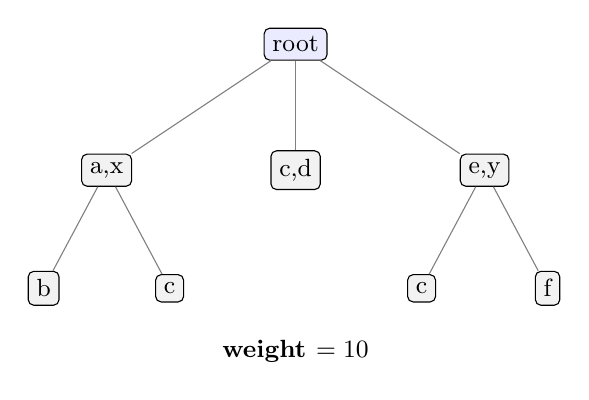
\begin{tikzpicture}[
nd/.style={draw, rounded corners=2pt, fill=black!5, inner sep=3pt, font=\small},
rt/.style={draw, rounded corners=2pt, fill=blue!8, inner sep=3pt, font=\small},
ed/.style={-, gray}
]
\node[rt] (r)  at (0,0) {root};
\node[nd] (ax) at (-2.4,-1.6) {a,x};
\node[nd] (cd) at ( 0.0,-1.6) {c,d};
\node[nd] (ey) at ( 2.4,-1.6) {e,y};
\draw[ed] (r)--(ax); \draw[ed] (r)--(cd); \draw[ed] (r)--(ey);
\node[nd] (b)  at (-3.2,-3.1) {b};
\node[nd] (c1) at (-1.6,-3.1) {c};
\node[nd] (c2) at ( 1.6,-3.1) {c};
\node[nd] (f)  at ( 3.2,-3.1) {f};
\draw[ed] (ax)--(b); \draw[ed] (ax)--(c1);
\draw[ed] (ey)--(c2); \draw[ed] (ey)--(f);
\node[font=\small\bfseries] at (0,-3.9) {weight $= 10$};
\end{tikzpicture}}
\end{center}
Greedy gives $12$, the optimum here is $10$ --- and we know of no
efficient algorithm for the optimum.
\end{frame}

%======================================================================
%  PART VI  --  Path indexing
%======================================================================
\section{Path indexing}

%--- Motivation -------------------------------------------------------
\begin{frame}{Path indexing: storing sets of expressions}
  \begin{itemize}
    \item Like \alert{discrimination trees}, a path index stores a set of
          syntax trees (\texttt{Expr})
    \item Used for efficient membership queries
    \item Each stored expression gets an \alert{index}; the tree mirrors the
          shape of \texttt{Expr}, and every node records \alert{which indices
          carry which symbol} at that position.
    \item Will lead to \alert{scoring heuristic} of the next section.
  \end{itemize}
\end{frame}

%--- Path index tree (MaRDI slide 15, corrected) ----------------------
\begin{frame}{One index for three statements}
  \begin{center}
  \resizebox{!}{6cm}{%
  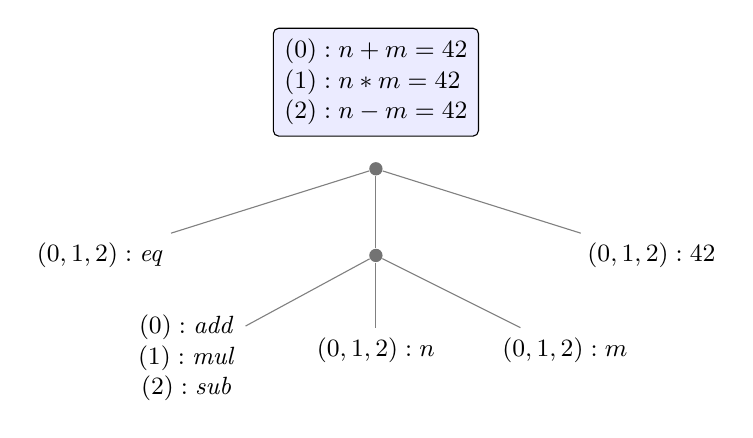
\begin{tikzpicture}[
    stmt/.style={draw, rounded corners=2pt, fill=blue!8, align=left,
                 inner sep=4pt, font=\small},
    app/.style={circle, fill=black!55, inner sep=1.7pt},
    lf/.style={font=\small, align=center},
    ed/.style={-, gray}
  ]
    \node[stmt] (S) at (0,1.5)
      {$(0) : n + m = 42$\\ $(1) : n * m = 42$\\ $(2) : n - m = 42$};
    % top application node
    \node[app] (A1) at (0,0.4) {};
    \node[lf]  (eq) at (-3.5,-0.7) {$(0,1,2) : \mathit{eq}$};
    \node[app] (A2) at (0,-0.7) {};
    \node[lf]  (l42) at (3.5,-0.7) {$(0,1,2) : 42$};
    \draw[ed] (A1)--(eq); \draw[ed] (A1)--(A2); \draw[ed] (A1)--(l42);
    % children of the inner application node (siblings)
    \node[lf] (op) at (-2.4,-2.0)
      {$(0) : \mathit{add}$\\ $(1) : \mathit{mul}$\\ $(2) : \mathit{sub}$};
    \node[lf] (n)  at (0,-1.9) {$(0,1,2) : n$};
    \node[lf] (m)  at (2.4,-1.9) {$(0,1,2) : m$};
    \draw[ed] (A2)--(op); \draw[ed] (A2)--(n); \draw[ed] (A2)--(m);
  \end{tikzpicture}}
  \end{center}
\end{frame}

%--- Query walkthrough, depth 1 ---------------------------------------
\begin{frame}{Querying for membership: $n + m = 42$ \hfill (depth 1)}
  \begin{center}
  \resizebox{!}{4.3cm}{%
  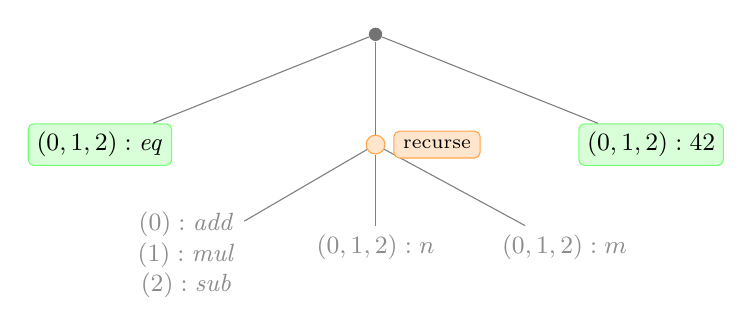
\begin{tikzpicture}[
    app/.style={circle, fill=black!55, inner sep=1.7pt},
    lf/.style={font=\small, align=center, inner sep=3pt, rounded corners=2pt},
    ed/.style={-, gray},
    hit/.style={fill=green!15, draw=green!55},
    rec/.style={fill=orange!20, draw=orange!70},
    dim/.style={text=black!45}
  ]
    \node[app] (A1) at (0,0.6) {};
    \node[lf,hit] (eq)  at (-3.5,-0.8) {$(0,1,2) : \mathit{eq}$};
    \node[app,rec,circle,inner sep=2.4pt] (A2) at (0,-0.8) {};
    \node[lf,hit] (l42) at (3.5,-0.8) {$(0,1,2) : 42$};
    \draw[ed] (A1)--(eq); \draw[ed] (A1)--(A2); \draw[ed] (A1)--(l42);
    \node[lf,dim] (op) at (-2.4,-2.2)
      {$(0) : \mathit{add}$\\ $(1) : \mathit{mul}$\\ $(2) : \mathit{sub}$};
    \node[lf,dim] (n)  at (0,-2.1) {$(0,1,2) : n$};
    \node[lf,dim] (m)  at (2.4,-2.1) {$(0,1,2) : m$};
    \draw[ed] (A2)--(op); \draw[ed] (A2)--(n); \draw[ed] (A2)--(m);
    \node[rec, rounded corners=2pt, font=\scriptsize, right=1mm of A2] {recurse};
  \end{tikzpicture}}
  \end{center}
  Split $n+m=42  \equiv{eq}\,(n+m)\,42$. The head $\mathit{eq}$ and the literal
  $42$ each match \alert{all} indices, $\{0,1,2\}$; the middle argument $n+m$
  needs a \alert{recursion}.
\end{frame}

%--- Query walkthrough, depth 2 ---------------------------------------
\begin{frame}{Querying for membership: $n + m = 42$ \hfill (depth 2)}
  \begin{center}
  \resizebox{!}{4.3cm}{%
  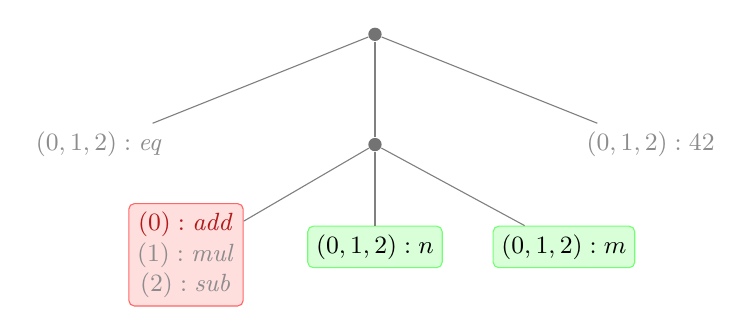
\begin{tikzpicture}[
    app/.style={circle, fill=black!55, inner sep=1.7pt},
    lf/.style={font=\small, align=center, inner sep=3pt, rounded corners=2pt},
    ed/.style={-, gray},
    hit/.style={fill=green!15, draw=green!55},
    restr/.style={fill=red!13, draw=red!60},
    dim/.style={text=black!45}
  ]
    \node[app] (A1) at (0,0.6) {};
    \node[lf,dim] (eq)  at (-3.5,-0.8) {$(0,1,2) : \mathit{eq}$};
    \node[app] (A2) at (0,-0.8) {};
    \node[lf,dim] (l42) at (3.5,-0.8) {$(0,1,2) : 42$};
    \draw[ed] (A1)--(eq); \draw[ed] (A1)--(A2); \draw[ed] (A1)--(l42);
    \node[lf,restr] (op) at (-2.4,-2.2)
      {${\color{keywordcolor}(0) : \mathit{add}}$\\
       ${\color{black!45}(1) : \mathit{mul}}$\\
       ${\color{black!45}(2) : \mathit{sub}}$};
    \node[lf,hit] (n)  at (0,-2.1) {$(0,1,2) : n$};
    \node[lf,hit] (m)  at (2.4,-2.1) {$(0,1,2) : m$};
    \draw[ed] (A2)--(op); \draw[ed] (A2)--(n); \draw[ed] (A2)--(m);
  \end{tikzpicture}}
  \end{center}
  In the recursion, $n$ and $m$ both match $\{0,1,2\}$, but the head
  $\mathit{add}$ matches \alert{only $\{0\}$}. Intersecting:
  $\{0,1,2\}\cap\{0,1,2\}\cap\{0\} = \{0\}$.
\end{frame}

%--- Query walkthrough, final -----------------------------------------
\begin{frame}{Querying for membership: $n + m = 42$ \hfill (result)}
  \begin{center}
  \resizebox{!}{3.4cm}{%
  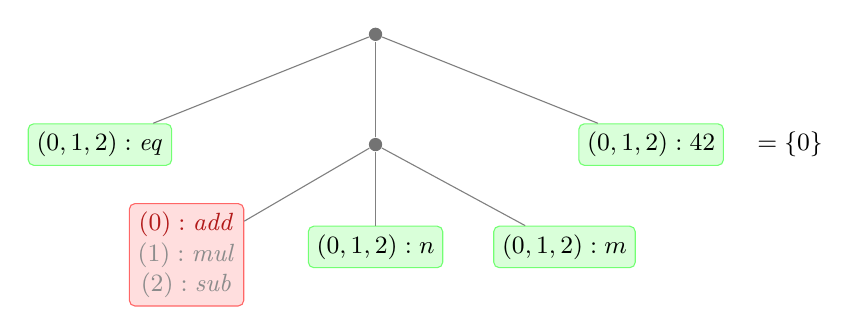
\begin{tikzpicture}[
    app/.style={circle, fill=black!55, inner sep=1.7pt},
    lf/.style={font=\small, align=center, inner sep=3pt, rounded corners=2pt},
    ed/.style={-, gray},
    hit/.style={fill=green!15, draw=green!55},
    restr/.style={fill=red!13, draw=red!60}
  ]
    \node[app] (A1) at (0,0.6) {};
    \node[lf,hit] (eq)  at (-3.5,-0.8) {$(0,1,2) : \mathit{eq}$};
    \node[app] (A2) at (0,-0.8) {};
    \node[lf,hit] (l42) at (3.5,-0.8) {$(0,1,2) : 42$};
    \draw[ed] (A1)--(eq); \draw[ed] (A1)--(A2); \draw[ed] (A1)--(l42);
    \node[lf,restr] (op) at (-2.4,-2.2)
      {${\color{keywordcolor}(0) : \mathit{add}}$\\
       ${\color{black!45}(1) : \mathit{mul}}$\\
       ${\color{black!45}(2) : \mathit{sub}}$};
    \node[lf,hit] (n)  at (0,-2.1) {$(0,1,2) : n$};
    \node[lf,hit] (m)  at (2.4,-2.1) {$(0,1,2) : m$};
    \draw[ed] (A2)--(op); \draw[ed] (A2)--(n); \draw[ed] (A2)--(m);
    \node[font=\small\bfseries, right=3mm of l42] {$= \{0\}$};
  \end{tikzpicture}}
  \end{center}
  Back at the root: $\underbrace{\{0,1,2\}}_{\mathit{eq}} \cap
  \underbrace{\{0\}}_{n+m} \cap \underbrace{\{0,1,2\}}_{42} = \{0\}$ ---
  so $n+m=42$ is stored, at index $0$.

\end{frame}

%--- Path index tree Aspects ----------------------
\begin{frame}{Aspects}
\begin{center}
	\resizebox{!}{4cm}{%
		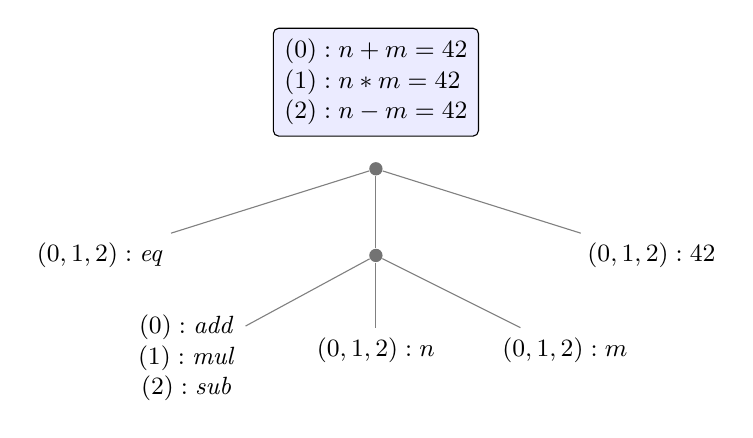
\begin{tikzpicture}[
			stmt/.style={draw, rounded corners=2pt, fill=blue!8, align=left,
				inner sep=4pt, font=\small},
			app/.style={circle, fill=black!55, inner sep=1.7pt},
			lf/.style={font=\small, align=center},
			ed/.style={-, gray}
			]
			\node[stmt] (S) at (0,1.5)
			{$(0) : n + m = 42$\\ $(1) : n * m = 42$\\ $(2) : n - m = 42$};
			% top application node
			\node[app] (A1) at (0,0.4) {};
			\node[lf]  (eq) at (-3.5,-0.7) {$(0,1,2) : \mathit{eq}$};
			\node[app] (A2) at (0,-0.7) {};
			\node[lf]  (l42) at (3.5,-0.7) {$(0,1,2) : 42$};
			\draw[ed] (A1)--(eq); \draw[ed] (A1)--(A2); \draw[ed] (A1)--(l42);
			% children of the inner application node (siblings)
			\node[lf] (op) at (-2.4,-2.0)
			{$(0) : \mathit{add}$\\ $(1) : \mathit{mul}$\\ $(2) : \mathit{sub}$};
			\node[lf] (n)  at (0,-1.9) {$(0,1,2) : n$};
			\node[lf] (m)  at (2.4,-1.9) {$(0,1,2) : m$};
			\draw[ed] (A2)--(op); \draw[ed] (A2)--(n); \draw[ed] (A2)--(m);
	\end{tikzpicture}}
\end{center}

  \begin{itemize}
	\item Matching is done \alert{up to reduction} ($2+2$ should match $4$):
	      \\we handle this with normal forms and partial builds.
	\item And \alert{up to unification}: nodes may carry metavariables, so a query
	can retrieve every stored expression it \emph{unifies} with, not only
	the syntactically identical one.
	\\Ex.: if $n$ is a metavariable, match $(a*b)+m=42$ with assignment
	\\These assignements must be tracked/propagated !
\end{itemize}

\end{frame}

%======================================================================
%  PART VII  --  The search heuristic
%======================================================================
\section{The search heuristic}

%--- The memorisation idea --------------------------------------------
\begin{frame}{A memorisation heuristic for steps}
  \begin{block}{Task}
    During the search: is applying \alert{this theorem} a good next step?
  \end{block}
  \medskip
  \begin{itemize}
    \item From a \alert{library of proofs}: every time a theorem is applied, record
          the proof state --- its \alert{goal} and the \alert{local hypotheses}
          present.
    \item \alert{Memorisation.} A theorem is a promising candidate when, in
          \grow{}'s current state,
      \begin{itemize}
        \item the search goal \emph{matches} a recorded goal, and
        \item the search context \emph{contains} the recorded hypotheses.
      \end{itemize}
    \item The recorded goals/context get \alert{generalised} with a path-index procedure --- \emph{covered later}.
  \end{itemize}
  \medskip
  So the first task is to \alert{sample proof states} from proofs.
\end{frame}

%--- The source proof we sample from ----------------------------------
\begin{frame}[fragile]{Sampling proof states}
  We replay a proof and, at \alert{each theorem application}, emit a sample.
\begin{lstlisting}
theorem testProof (l L : List Nat) :
    l.dedup.dedup.length + L.length ≤ (l ++ L).length := by
  rw [dedup_idem, length_append]
  apply Nat.add_le_add_right
  apply Sublist.length_le
  apply dedup_sublist
\end{lstlisting}
  A sample records the \alert{goal} and the
  \alert{hypotheses} it relied on, and the \alert{theorem} applied.
\end{frame}

%--- A few samples ----------------------------------------------------
\begin{frame}[fragile]{A few samples from that proof}
\begin{lstlisting}[basicstyle=\ttfamily\small]
	Goal:  l.dedup.length ≤ l.length
	Hyps:  (none)
	Kind:  thm List.Sublist.length_le
\end{lstlisting}
Directly from proof:
\begin{lstlisting}
theorem testProof (l L : List Nat) :
	l.dedup.dedup.length + L.length ≤ (l ++ L).length := by
  rw [dedup_idem, length_append]
  apply Nat.add_le_add_right
  -- sampled here
  apply Sublist.length_le
  apply dedup_sublist
\end{lstlisting}
\end{frame}


%--- A few samples ----------------------------------------------------
\begin{frame}[fragile]{A few samples from that proof}
\begin{lstlisting}[basicstyle=\ttfamily\small]
	Goal:  l.dedup.length + L.length ≤ l.length + L.length
	Hyps:  l.dedup <+ l
	Kind:  thm Nat.add_le_add_right
\end{lstlisting}
One proof terms, many derivations. Sample ficticious foward step:
\begin{lstlisting}
theorem testProof (l L : List Nat) :
	l.dedup.dedup.length + L.length ≤ (l ++ L).length := by
  rw [dedup_idem, length_append]
  have ficticous := dedup_sublist l
  -- ficticious foward step
  -- sample here
  apply Nat.add_le_add_right
  apply Sublist.length_le
  apply ficticous
\end{lstlisting}
\end{frame}

%--- Conjecturables ---------------------------------------------------
%\begin{frame}[fragile]{Conjecturables: arguments the goal doesn't reveal}
%Consider a transitivity step:
%\begin{lstlisting}[basicstyle=\ttfamily\scriptsize]
%theorem testConj (n m : Nat) : n*m + 1 ≤ 2 + (m*n) := by
%  calc n*m + 1 = m*n + 1   := by rw [Nat.mul_comm]
%    _          = 1 + (m*n) := by rw [Nat.add_comm]
%    _          ≤ 2 + (m*n) := by apply Nat.add_le_add_right; decide
%\end{lstlisting}
%\begin{lstlisting}[basicstyle=\ttfamily\small]
%Goal:  n * m + 1 = 1 + m * n
%Hyps:  · n * m + 1 = m * n + 1
%Kind:  thmC Eq.trans #[m * n + 1]
%\end{lstlisting}
%  \begin{itemize}
%    \item \texttt{Eq.trans} transitions through $m*n+1$ --- a term the goal
%          $n*m+1 = 1+m*n$ \alert{does not mention}, so it cannot be inferred from it.
%    \item We track such \alert{conjecturable} arguments (\texttt{\#[m * n + 1]}),
%          for better-informed backward steps.
%  \end{itemize}
%\end{frame}

%--- Generalisation: the procedure ------------------------------------
\begin{frame}{From samples to a pattern: generalisation}
We can do better then memorisation.
\\For each theorem, we merge all its recorded goals into \alert{one path index}, then \alert{generalise} it:
  \medskip
  \begin{itemize}
    \item Leave \alert{frequent} sub-expressions as they are.
    \item For \alert{infrequent} ones, infer their type and look for a
          \alert{frequent type}.
    \item Replace an infrequent expression by a \alert{metavariable} of that type.
  \end{itemize}
  \medskip
  A search goal then counts as \emph{resembling} the samples when it
  \alert{unifies} with this pattern
\end{frame}

%--- Generalisation: reminder of the initial index --------------------
\begin{frame}{Reminder: the recorded goals, as one path index}
\begin{center}
  \resizebox{!}{6cm}{%
  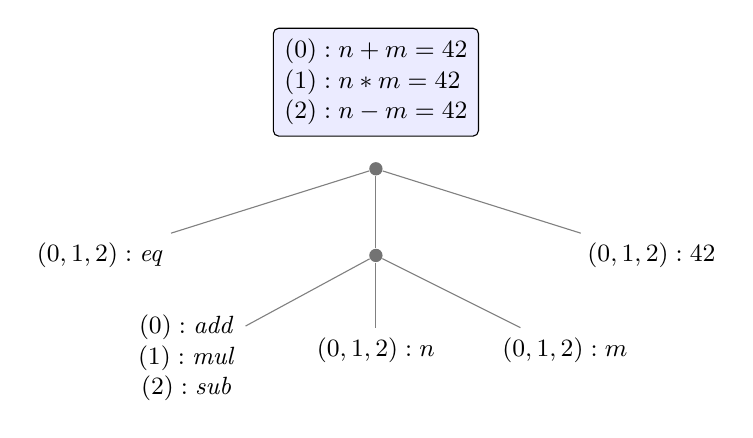
\begin{tikzpicture}[
    stmt/.style={draw, rounded corners=2pt, fill=blue!8, align=left,
                 inner sep=4pt, font=\small},
    app/.style={circle, fill=black!55, inner sep=1.7pt},
    lf/.style={font=\small, align=center},
    ed/.style={-, gray}
  ]
    \node[stmt] (S) at (0,1.5)
      {$(0) : n + m = 42$\\ $(1) : n * m = 42$\\ $(2) : n - m = 42$};
    \node[app] (A1) at (0,0.4) {};
    \node[lf]  (eq) at (-3.5,-0.7) {$(0,1,2) : \mathit{eq}$};
    \node[app] (A2) at (0,-0.7) {};
    \node[lf]  (l42) at (3.5,-0.7) {$(0,1,2) : 42$};
    \draw[ed] (A1)--(eq); \draw[ed] (A1)--(A2); \draw[ed] (A1)--(l42);
    \node[lf] (op) at (-2.4,-2.0)
      {$(0) : \mathit{add}$\\ $(1) : \mathit{mul}$\\ $(2) : \mathit{sub}$};
    \node[lf] (n)  at (0,-1.9) {$(0,1,2) : n$};
    \node[lf] (m)  at (2.4,-1.9) {$(0,1,2) : m$};
    \draw[ed] (A2)--(op); \draw[ed] (A2)--(n); \draw[ed] (A2)--(m);
  \end{tikzpicture}}

\end{center}
 {\footnotesize Here, we call a pattern \alert{infrequent} when it occurs in \alert{$\leq \tfrac{1}{3}$} of its siblings.}  
\end{frame}

%--- Generalisation: the generalised index ----------------------------
\begin{frame}{Generalising the index}
  \begin{center}
  \resizebox{!}{5.4cm}{%
  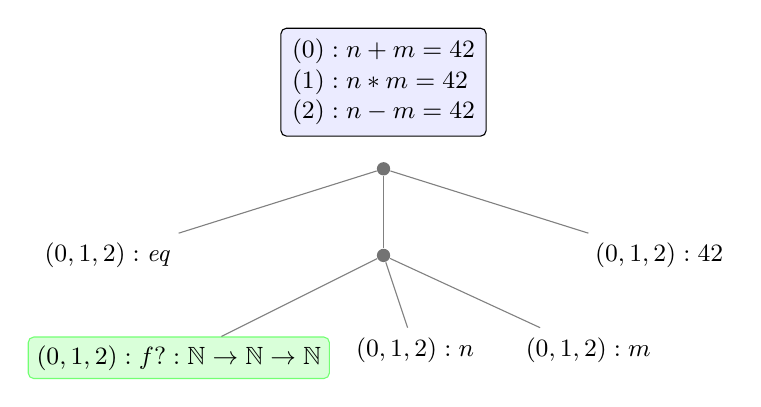
\begin{tikzpicture}[
    stmt/.style={draw, rounded corners=2pt, fill=blue!8, align=left,
                 inner sep=4pt, font=\small},
    app/.style={circle, fill=black!55, inner sep=1.7pt},
    lf/.style={font=\small, align=center},
    gen/.style={font=\small, align=center, rounded corners=2pt,
                fill=green!15, draw=green!55, inner sep=3pt},
    ed/.style={-, gray}
  ]
    \node[stmt] (S) at (0,1.5)
      {$(0) : n + m = 42$\\ $(1) : n * m = 42$\\ $(2) : n - m = 42$};
    \node[app] (A1) at (0,0.4) {};
    \node[lf]  (eq) at (-3.5,-0.7) {$(0,1,2) : \mathit{eq}$};
    \node[app] (A2) at (0,-0.7) {};
    \node[lf]  (l42) at (3.5,-0.7) {$(0,1,2) : 42$};
    \draw[ed] (A1)--(eq); \draw[ed] (A1)--(A2); \draw[ed] (A1)--(l42);
    \node[gen] (op) at (-2.6,-2.0) {$(0,1,2) : f? :\mathbb{N}\to \mathbb{N}\to\mathbb{N}$};
    \node[lf]  (n)  at ( 0.4,-1.9) {$(0,1,2) : n$};
    \node[lf]  (m)  at ( 2.6,-1.9) {$(0,1,2) : m$};
    \draw[ed] (A2)--(op); \draw[ed] (A2)--(n); \draw[ed] (A2)--(m);
  \end{tikzpicture}}
  \end{center}
  Each of \textit{add}, \textit{mul}, \textit{sub} occurs in just
  $\tfrac{1}{3}$ of the siblings --- \alert{infrequent} --- so they collapse to a
  metavariable $f? : \mathbb{N}\to\mathbb{N}\to\mathbb{N}$. $n/m=42$ will now match !
\end{frame}

%--- Generalisation: aspects and status -------------------------------
\begin{frame}[fragile]{Generalisation: open aspects}
  \begin{itemize}
    \item \alert{Metavariable garbage collection}: Generalisation can create
          metavariables that later get generalised further and are no longer
          referenced by the index --- these can be removed.
    \item \alert{Metavariable reuse}: We want as few metavariables as possible for efficiency (keep path indices small): no need to have two $(m? \ :  \mathbb{N})$ if no goals share them.
          \\This is delicate and \alert{still in a research state}.
    \item \alert{On real data.} Running the procedure over a larger body of
          samples:
\begin{lstlisting}[basicstyle=\ttfamily\footnotesize]
-- 6_Heuristic.lean, line 56
#eval explore_gen_thm_core_S
  `LeanGrow.Src.Caching.Score.Test.DummySamples
\end{lstlisting}
          \ldots the output is, frankly, \alert{quite hard to see through}.
  \end{itemize}
\end{frame}

%======================================================================
%  PART VIII  --  Closing words
%======================================================================
\section{Closing words}

%--- Placeholder to be filled in --------------------------------------
\begin{frame}{Closing words}

\begin{itemize}
	\item Heuristic proof search can't compete with LLMs \\\dots for now. But maybe one day ?
	\item Currently a \alert{statistical/phenomenological} approach: take theorem as search step if goal and context match previously seen  frequent applications.
	\\Move towards \alert{learning}: determine goal path index and context set-trie that \textit{minimise} search step count or proof term size for a given set of target queries. How ?
	\item Work in progress: rewrite with dependent constants ? Link induction reverts to samples ? Optimal set-tries and fuzzy queries ? Sample tactic applications ? Move to Aesop. Fix bugs. Optimize. Fix more bugs. 

\end{itemize}

\end{frame}

%--- Thanks -----------------------------------------------------------
\begin{frame}[plain,noframenumbering]
  \centering
  \vfill
  {\color{keywordcolor}\Huge\bfseries Thank you for your attention!}\par
  \vspace{1.2em}
  {\large Questions?}
  \vfill
\end{frame}

\end{document}
